\documentclass{beamer}
\usepackage[utf8]{inputenc}
\usepackage{xeCJK}
% 设置英文默认字体
\setmainfont{Times New Roman} 
% 设置中文默认字体
\setCJKmainfont[BoldFont=宋体-简 粗体]{宋体-简}
\usepackage{hyperref}
% \usepackage{cite}
\usepackage[backend=bibtex, sorting=none]{biblatex}
\addbibresource{Biblio/ref}
\setbeamertemplate{bibliography item}[text]
\usetheme{Madrid}
\usecolortheme{default}
\usepackage{tikz}
\usepackage{graphicx}
\usepackage{pgfplots}
\usetikzlibrary{shadows}
\usetikzlibrary{patterns} %填充
\usetikzlibrary{
        matrix,
    }
\usepackage{booktabs}
\usepackage{dcolumn}
\usepackage{siunitx}
%------------------------------------------------------------
%This block of code defines the information to appear in the
%Title page
\title[三角形计数] %optional
{三角形计数算法调研}

\subtitle{从精确算法到近似算法}

\author[刘丁玮] % (optional)
{刘丁玮}

% \institute[ICT] % (optional)
% {
%   \inst{1}%
%   Faculty of Physics\\
%   Very Famous University
%   \and
%   \inst{2}%
%   Faculty of Chemistry\\
%   Very Famous University
% }

\date[2022-06-30] % (optional)
{202218013229010}

% \logo{\includegraphics[height=1cm]{overleaf-logo}}

%End of title page configuration block
%------------------------------------------------------------



%------------------------------------------------------------
%The next block of commands puts the table of contents at the 
%beginning of each section and highlights the current section:

\AtBeginSection[]
{
  \begin{frame}
    \frametitle{目录}
    \tableofcontents[currentsection]
  \end{frame}
}
%------------------------------------------------------------


\begin{document}

%The next statement creates the title page.
\frame{\titlepage}

%---------------------------------------------------------
%This block of code is for the table of contents after
%the title page
\begin{frame}
\frametitle{目录}
\tableofcontents
\end{frame}
%---------------------------------------------------------
\section{介绍} 
\begin{frame}
\frametitle{介绍} 
图
\begin{itemize}
    \item 建模实体关系
    \item 社交网络、通信网络、生物网络等
\end{itemize}

三角形
\begin{itemize}
    \item 重要拓扑结构 
    \item 集聚性、同质性、传递性等
\end{itemize}
\end{frame}

\begin{frame}
\frametitle{三角形计数} 
任务
\begin{itemize}
    \item 统计三角形数量
    \item 枚举三角形并统计数量
\end{itemize}
应用
\begin{itemize}
    \item 网络垃圾邮件检测\cite{becchetti2008efficient}
    \item 数据库查询优化\cite{bar2002reductions}
    \item $\cdots$
\end{itemize}
挑战
\begin{itemize}
    \item 计算复杂度高,大规模场景开销巨大
    \item 图的偏斜分布\cite{barabasi1999emergence}导致相同复杂度的算法性能差异大
\end{itemize}
\end{frame}


\section{背景}
\begin{frame}
\frametitle{基本定义}
符号
\begin{table}
    \begin{tabular}[]{l|l} 
           \hline 
           $G,V,E,n,m$ & 图、节点集、边集、节点数$|V|$、边数$|E|$\\
           $u,e=(u,v)$ & 节点,边\\
           $d(u),d_{\max},adj(u)$ & $u$的度,图中最大的度、$u$的邻居节点集合\\
           $\Pi , \Pi^\angle, \Pi^\vartriangle$  & 三元组集合、三链集合、三角形集合\\
           \hline 
    \end{tabular}
\end{table}
三元组、三角形与三链
\begin{itemize}
    \item 三元组$<u,v,w>$是以$v$为中心的长度为2的路径。
    \item 如果$uw$也有边相连,构成闭三元组,称为三角形。
    \item 如果$uw$没有边相连,构成开三元组,称为三链。
\end{itemize}

\begin{figure}[H]
    \begin{tikzpicture}[font=\tiny]
        \draw [-,mark=*,mark size=2pt, fill=white] plot coordinates{(0,0)} -- plot coordinates{(2,0)} -- plot coordinates{(1,1)} -- plot coordinates{(0,0)}; 
        \draw [-,mark=*,mark size=2pt, fill=white] plot coordinates{(3,0)} -- plot coordinates{(5,0)} -- plot coordinates{(4,1)}; 
        \node at([yshift=-5pt]1,0) {三角形};
        \node at([yshift=5pt]0,0) {u};
        \node at([yshift=5pt]2,0) {v};
        \node at([yshift=5pt]1,1) {w};
        \node at([yshift=5pt]3,0) {u};
        \node at([yshift=5pt]5,0) {v};
        \node at([yshift=5pt]4,1) {w};
        \node at([yshift=-5pt]4,0) {三链};
    \end{tikzpicture}
\end{figure}
\end{frame}

\begin{frame}
\frametitle{基本定义}
$\Pi^\vartriangle $中三角形的不同节点贡献不同的三元组。
$\Lambda$表示图$G$中不同三角形的集合。三角形个数
\begin{equation}
    t(G)=|\Lambda|=\frac{1}{3}|\Pi^\vartriangle|=\frac{1}{3}\sum_{v\in V}|\Pi^\vartriangle_v|
    \label{eq:triangle_num}
\end{equation}
\begin{itemize}
\item 当且仅当图为全连接时,图中三角形数量最多,为$\left(\begin{array}{l}n \\3\end{array}\right)$。\\
\item 从点的角度考虑,$t(G)=O(n^{3})$。\\
\item 从边的角度考虑,$t(G)=O(m^{\frac{3}{2}})$。
\end{itemize}
\end{frame}


\begin{frame}
\frametitle{指标}
传递率
\begin{itemize}
\item 三角形与三元组总数的比值,记为$\gamma(G)$
\begin{equation}
    \gamma(G)=\frac{|\Pi^\vartriangle|}{|\Pi|}=\frac{\Pi^\vartriangle}{\Pi^\vartriangle+\Pi^\angle}
    \label{eq:transitivity}
\end{equation}
\item $t(G)$可以从其传递率计算,
\begin{equation}
    t(G)=\frac{1}{3}\cdot \gamma(G) \cdot |\Pi| 
    \label{eq:tc_trans}
\end{equation}
\end{itemize}
\end{frame}

\section{精确算法}
\begin{frame}
\frametitle{精确算法} 
最简单的算法
\begin{itemize}
    \item 枚举三节点集,检测是否构成三角形。
    \item $O(n^3)$
\end{itemize}
计数算法(不枚举)
\begin{itemize}
    \item 基于邻接矩阵乘
    \item $t(G)=\frac{1}{6}\text{Tr}(A^{3})$
    \item $O(n^{\omega})$,$\omega$最低2.373\cite{le2014powers}。
\end{itemize}
\begin{block}{AYZ算法\cite{alon1997finding}}
% $O(m^{\frac{2\omega}{\omega +1}})$ 
节点集划分为$V_{\text {low }}=\{v \in V: \mathrm{d}(v) \leq \beta\}$和$V_{\text {high }}=V \backslash V_{\text {low }}$。
$\beta=m^{\omega-1 / \omega+1}$。
\begin{itemize}
\item 对于$V_\text{low}$,至多$m \cdot \beta$条路径能构成三角形,复杂度为$O(m \beta)$。
\item 对于$V_\text{high}$,讨论至多$2m/ \beta$个节点,复杂度为$O((m/ \beta)^{\omega})$。
\end{itemize}
时间复杂度为$O( m^{\frac{2\omega}{\omega +1}})$。
$\omega = 3$时,为$O(m^{\frac{3}{2}})$。
\end{block}
枚举算法
\end{frame}

\begin{frame}
\frametitle{枚举算法}
Itai等(1978)提出的早期算法\parencite{itai1978finding}
\begin{columns}
\column{0.6\textwidth}
\begin{itemize}
    \item 流程
    \begin{itemize} 
        \item 构造图$G(V,E)$的生成树$T(V,E_{T})$
        \item $E_{T}$的每条边$(u,v)$,检查$(\text{pred}(u),v) \in E$?$(\text{pred}(v),u) \in E$?
        % 这个过程将$T$中所有边所在的全部三角形进行了枚举。
        \item 删除$T$的所有边更新$G$
        \item 迭代上述三步直到图中没有边
    \end{itemize}
    \item $O(m^\frac{3}{2})$
    \item 需要修改图数据结构,实际开销很高
\end{itemize}
\column{0.4\textwidth}
\begin{figure}[H]
    \begin{tikzpicture}[font=\tiny]
        \begin{scope}[xshift=-10cm]
            \draw [dashed] (-1,1) -- (0,0); 
            \draw [dashed] (0,2) -- (1,1); 
            \draw [-,mark=*,mark size=2pt, fill=white] plot coordinates{(-1,1)} -- plot coordinates{(0,2)} -- plot coordinates{(0,0)} -- plot coordinates{(1,1)}; 
            \node at([yshift=5pt]0,2) {u};
            \node at([yshift=-5pt]0,0) {v};
            \node at([xshift=15pt]1,1) {pred(v)};
            \node at([xshift=-15pt]-1,1) {pred(u)};
        \end{scope}
    \end{tikzpicture}
\end{figure}
\end{columns}
\end{frame}

\begin{frame}
\frametitle{枚举算法}
\begin{columns}
\column{0.6\textwidth}
节点迭代
\begin{itemize}
    \item 每个节点,检测任意两个不同邻居是否有边
    \item $\sum_{v\in V}\left(\begin{array}{l}d(v) \\2\end{array}\right)$,$O(nd^{2}_{\max})$
\end{itemize}
\column{0.4\textwidth}
\begin{figure}[H]
    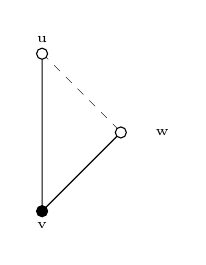
\begin{tikzpicture}[font=\tiny]
        \begin{scope}
            \draw [dashed] (0,2) -- (1,1); 
            \draw [-,mark=*,mark size=2pt, fill=white] plot coordinates{(0,2)} -- (0,0) -- plot coordinates{(1,1)}; 
            \draw [-,mark=*,mark size=2pt] plot coordinates{(0,0)}; 
            \node at([yshift=5pt]0,2) {u};
            \node at([yshift=-5pt]0,0) {v};
            \node at([xshift=15pt]1,1) {w};
        \end{scope}
    \end{tikzpicture}
\end{figure}
\end{columns}

\begin{columns}
\column{0.6\textwidth}
边迭代
\begin{itemize}
    \item 每条边,检测两个端点的邻居的交集
    \item $O(m d_{max})$
\end{itemize}

\column{0.4\textwidth}
\begin{figure}[H]
    \begin{tikzpicture}[font=\tiny]
        \begin{scope}
            \draw [dashed] (0,2) -- (1,1); 
            \draw [dashed] (0,0) -- (1,1); 
            \draw [-,thick] (0,2) -- (0,0);
            \draw [-,mark=*,mark size=2pt, fill=white] plot coordinates{(1,1)}; 
            \draw [-,mark=*,mark size=2pt] plot coordinates{(0,0)}; 
            \draw [-,mark=*,mark size=2pt] plot coordinates{(0,2)}; 
            \node at([yshift=5pt]0,2) {u};
            \node at([yshift=-5pt]0,0) {v};
            \node at([xshift=15pt]1,1) {w};
        \end{scope}
    \end{tikzpicture}
\end{figure}
\end{columns}
\end{frame}

\begin{frame}
\frametitle{精确算法}
\begin{columns}
\column{0.5\textwidth}
\begin{table}
    \begin{tabular}{ll} 
           \multicolumn{2}{c}{\textbf{计数算法}} \\
           \midrule   
            $O(n^3)$&矩阵乘\\
            $O(n^\omega)$&快速矩阵乘\\
            $O(m^\frac{2\omega}{\omega +1})$&AYZ使用快速矩阵乘\\
    \end{tabular}
\end{table}
\column{0.4\textwidth}
\begin{table}
    \begin{tabular}{ll} 
           \multicolumn{2}{c}{\textbf{枚举算法}} \\
           \midrule   
            $O(n^3)$ & 简单枚举\\
            $O(nd_{\max}^2)$ & 节点迭代\\
            $O(md_{\max})$&边迭代\\
    \end{tabular}
\end{table}
\end{columns}
\begin{itemize}
    \item 最优的时间复杂度为$O( m^{\frac{2\omega}{\omega +1}})$,$\omega$最低2.373\cite{le2014powers}
    \item 枚举算法中避免冗余统计可以有效减少运行时间\cite{schank2005finding, latapy2008main}
    \item 对十亿级别边的图仍非常昂贵
\end{itemize}
\end{frame}

\section{近似算法}
\begin{frame}
\frametitle{近似算法} 

基于图稀疏化的三角形计数方法
    \begin{itemize}
    \item 三角形以均匀概率采样 
    \end{itemize}

基于三元组采样的三角形计数方法
    \begin{itemize}
    \item 三元组以均匀概率采样
    \end{itemize}

基于节点或边迭代法的三角形计数估计方法
    \begin{itemize}
    \item 节点、边以均匀概率采样
    \end{itemize}
\end{frame}

\begin{frame}
\frametitle{基于图稀疏化的三角形计数方法} 
思路
\begin{itemize}
    \item 随机删除图中的一个边子集,得到稀疏图
    \item 从稀疏图的精确三角形计数推算原始图三角形计数
\end{itemize}
\begin{block}{DOULION算法变体\cite{etemadi2016efficient}}
对给定图$G$的边以$p$的概率均匀采样,得到稀疏图$G_s$。统计$G_s$中三角形和$G$中对应的三元组是三角形的三链
\begin{itemize}
    \item 三角形的采样概率为$p^2$
    \item $\hat{t}(G)=\frac{1}{ p^{2}} \cdot t\left(G_{\mathrm{s}}\right)$
\end{itemize}
\end{block}
\end{frame}

\begin{frame}
\frametitle{基于三元组采样的三角形计数方法} 
思路
\begin{itemize}
    \item 均匀采样三元组,得到三元组集合$T$,计算传递率的无偏估计$\hat{\gamma}$
    \begin{equation}
        \hat{\gamma}=\frac{\sum_{t \in T} \mathbb{I}_{t \text { is closed }}}{|T|}
        \label{eq:app_trans}
    \end{equation}
    \item 使用$\hat{\gamma}$估算原始图三角形计数
\end{itemize}
\begin{block}{Schank等(2005a)提出的算法\cite{schank2005approximating}}
    先以概率$\frac{|\Pi_{v}|}{|\Pi|}$采样节点,再从得到的每个节点的三元组中随机返回一个,以$v$为中心的三元组随机返回概率为$\frac{1}{|\Pi_v|}$
    \begin{itemize}
        \item 三元组的采样概率为$\frac{1}{|\Pi|}$
        \item $\hat{t}(G)=\frac{1}{3} \cdot \hat{\gamma} \cdot|\Pi|$
    \end{itemize}
\end{block}
\end{frame}

\begin{frame}
\frametitle{基于节点或边迭代的三角形计数估计方法\cite{rahman2013approximate}} 

\begin{itemize}
    \item 采样部分节点或边,并统计它们所在三角形数量。
    \item 根据采样比例估算原始图三角形计数。
\end{itemize}

\begin{figure}[H]
    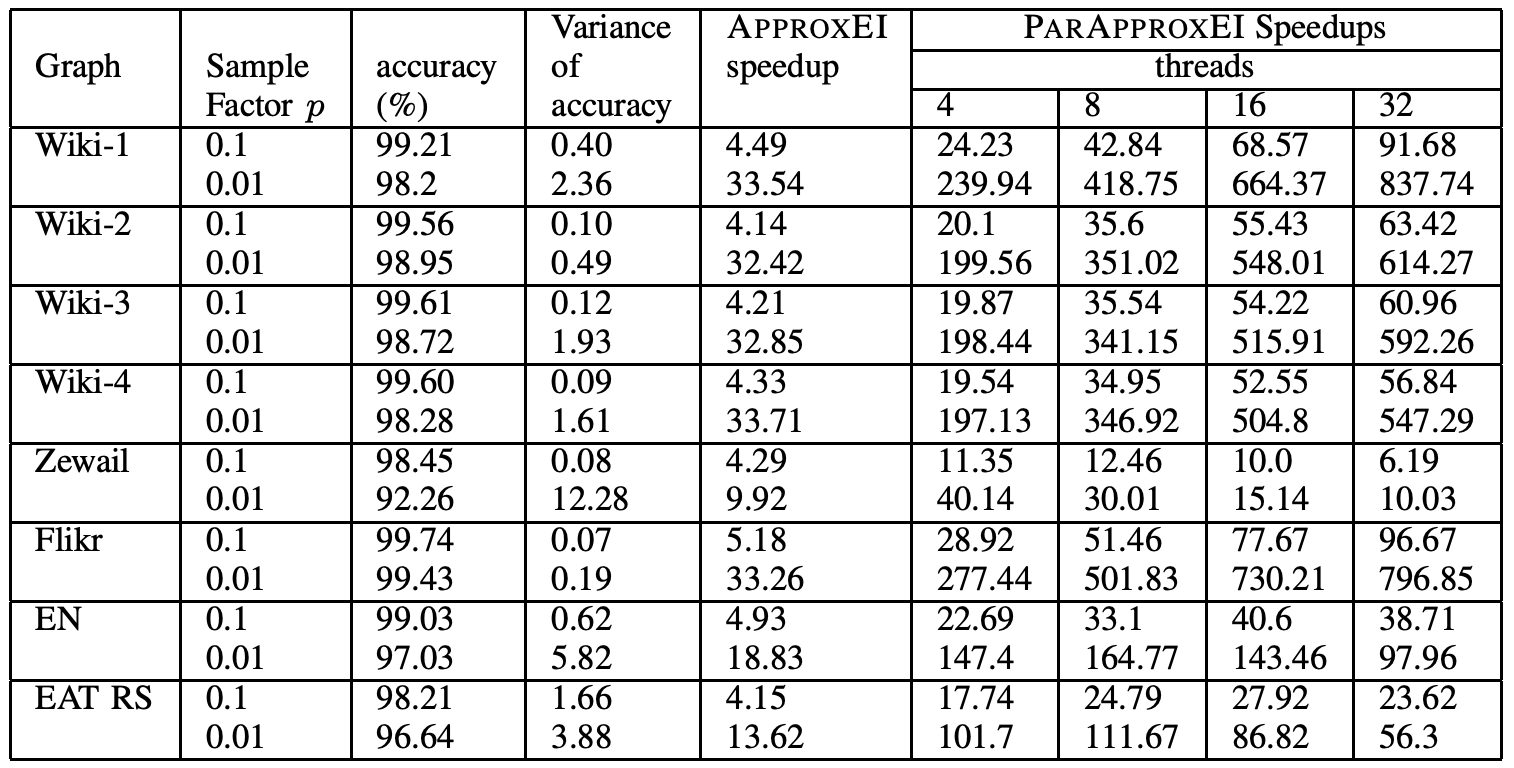
\includegraphics[width=\textwidth]{Img/tb.png}
\end{figure}
\end{frame}

\section{总结}
\begin{frame}
\frametitle{总结} 
\begin{itemize}
\item 三角形在图分析领域有着重要作用\\
\item 三角形计数和枚举是大图数据挖掘的重要任务、也可以作为更复杂分析任务的前置处理步骤\\
\item 通过算法设计和实现优化,三角形计数精确算法的实际运行开销降到了可接受的范围\\
\item 无需精确值的超大图场景下,近似算法有远超精确算法优越的性能\\
\end{itemize}
\end{frame}

\begin{frame}[allowframebreaks] 
\frametitle{参考文献}
    \printbibliography
\end{frame}
\end{document}